\chapter{Presentación de los datos, Análisis, Discusión}

En algunas disciplinas, el capítulo Presentación de datos va acompañado del análisis o de la discusión de la información (\textit{Presentación y análisis de los datos}; \textit{Resultados y discusión}), en tanto que en otras, \textit{Presentación}, \textit{Análisis} y \textit{Discusión} son capítulos separados.
El objetivo de esta(s) parte(s) de la tesis es presentar los datos recabados y el análisis realizado a la luz de la bibliografía ya revisada. Se puede incluir la interpretación de los resultados (\textit{Discusión}) a partir del análisis de los datos, o también relacionarlos con estudios relevantes que se entienden pertinentes, aun si estos no se han consignado en los \textit{Fundamentos teóricos}, ya que se entiende que al analizar los datos pueden aparecer algunos que no se enmarcan teóricamente o que no se explican en el encuadre teórico o en estudios ya existentes.

Ahora a modo de ejemplo mencionamos el símbolo de los números reales utilizando el comando \verb|\gls{}| \gls{Real} y el comando \verb|\glssymbol{}| \glssymbol{Real}. Otro ejemplo es mencionar el tensor simétrico de tensiones \gls{sigma}, o un valor escalar  \gls{alph} o un conjunto vacío \gls{emptyset}.

\newpage 
\section{Notas en el documento}

También se encuentra la posibilidad de colocar notas en la tesis, de manera muy simple. En este caso se soporta dos tipos de notas distintos,  una para el autor del documento y otra para el revisor. Con el comando \verb|\todo{texto}| el autor puede colocar una nota \todo{Nota del autor en el margen, en color verde}. Con el comando \verb|\revisor{texto}| el revisor de la tesis puede realizar una nota \revisor{Nota del revisor en color rojo}. El corrector debería recibir el archivo \verb|tesis.tex|, con todos los archivos dependientes de este para poder hacer los cambios  \todo{Otra nota del autor en el margen un poco más larga} y compilar la tesis. Otra opción es que editen simplemente el archivo del capítulo a revisar en cualquier editor de texto, sin compilar.

También se encuentra la posibilidad de colocar una nota que se encuentre dentro del párrafo con la opción \verb|inline|. \todo[inline]{Esto es un ejemplo de una nota dentro del párrafo} 
Si falta colocar una figura se puede indicar con el comando \verb|\missingfigure|.
\missingfigure{Gráfica de análisis.}

Con el comando \verb|\listoftodos| se puede insertar una lista con todas las notas colocadas en el documento, para facilitar la revisión.
\listoftodos

\section{Título de sección}

Ejemplo de tabla

\begin{table}[h!]
\centering
\caption{Leyenda de tabla.}
\label{tab:comp}
\begin{tabular}{|c|c|c|}
  \hline
  $t$ (seg) & $x$(t) & $y$(t)\\
  \hline
  1 & 0.0000 & 0.0001\\
  2 & 0.5000 & 0.2498\\
  3 & 1.0000 & 1.0000\\
  4 & 1.5000 & 2.2403\\
  5 & 2.0000 & 4.0010\\
  6 & 2.5000 & 6.2459\\
  \hline
\end{tabular}
\end{table}

Ejemplo de figura.

\begin{figure}[h!]
\label{fig:comp}
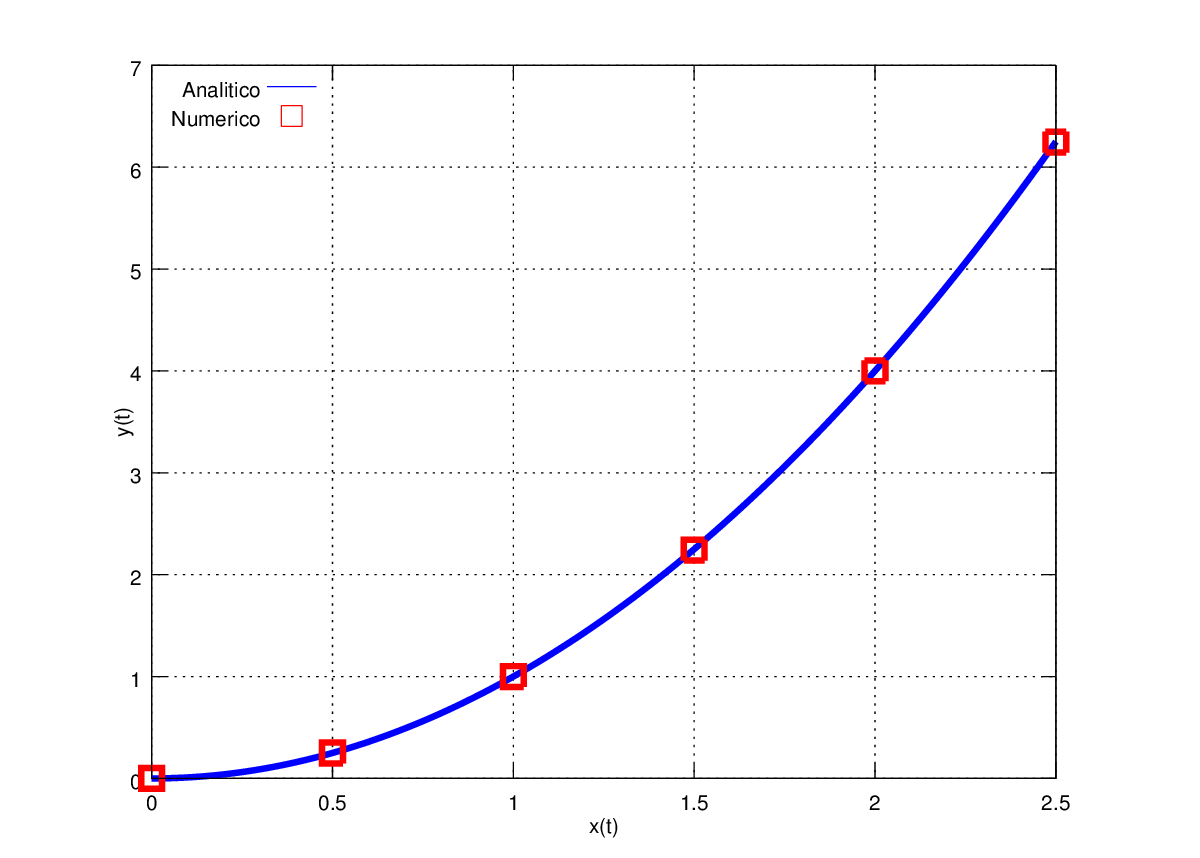
\includegraphics[width=.8\textwidth]{imagenes/chap4/x_vs_y}
\caption{Leyenda de figura.}
\end{figure}
Ejemplo de ecuación:
\begin{equation}
y(x)=x^2
\end{equation}
